%{
% \documentclass[12pt,ngerman]{/Users/dominik-cau/Documents/Lernen/Uni/Promotion/Vorlagen/Bayreuth/Exercise/AssignmentClass}
\documentclass[12pt,ngerman]{AssignmentClass}
% \documentclass{article}
%\documentclass[12pt, english]{AssignmentClass}


%----------------------------------------------------------------------------------------
%	PACKAGES AND OTHER DOCUMENT CONFIGURATIONS
%----------------------------------------------------------------------------------------
% Template-specific packages
\usepackage[utf8]{inputenc} % Required for inputting international characters
\usepackage[T1]{fontenc} % Output font encoding for international characters
\usepackage{mathpazo} % Use the Palatino font
\usepackage{wasysym} % for flash-symbol
\usepackage{graphicx} % Required for including images
\usepackage{amsmath}
\usepackage{listings} % Required for insertion of code
\usepackage{siunitx}
\usepackage{pnets}
\usepackage[most]{tcolorbox} % Grey Deadline Bar
\DeclareMathAlphabet{\mathpzc}{OT1}{pzc}{m}{it}
% Initialize comment sections
\usetheme{light-theme}
\excludecomment{dark-theme}
\excludecomment{solution}


%----------------------------------------------------------------------------------------
%	SET VERSION
%----------------------------------------------------------------------------------------
%\includecomment{dark-theme}
\includecomment{solution}


%----------------------------------------------------------------------------------------
%	ASSIGNMENT INFORMATION
%----------------------------------------------------------------------------------------
%\setlanguageEnglish
%\setlanguageGerman
% \begin{dark-theme}
% 	\usetheme{dark-theme}
% 	\excludecomment{light-theme}
% \end{dark-theme}
\title{Übung 3 Lösung} % Assignment title
\instructor{Yorck Zisgen}
\class{Generative Künstliche Intelligenz} % Course or class name
\term{Sommersemester 2024}
% \topics{Begriffe $\bullet$ Kontrollflussmuster $\bullet$ Organisationseinheiten}
\topics{10.06.2024}
%----------------------------------------------------------------------------------------
%}

\begin{document}
	\maketitle

    % Header Deadline Bar
    %{
    \noindent % Ensures the box spans the entire width
    \begin{tcolorbox}[colback=gray!20, % Background color as light gray
                      colframe=gray!20, % Frame color same as background
                      boxrule=0pt, % No border
                      sharp corners, % Sharp corners
                      valign=center, % Vertically centered text
                      halign=center, % Horizontally centered text
                      height=2cm] % Height of the box
    \LARGE \bfseries Beispiellösung % Bold text
    \end{tcolorbox}
    %}

    \section{Foundation Models}
        Stellen Sie sich ein Einzelhandelsunternehmen vor, das ein Foundation Model wie DALL-E verwendet, um maßgeschneiderte Marketingmaterialien auf Basis von Verbraucherverhaltensdaten zu erstellen. Analysieren Sie, wie die Verwendung dieses KI-Modells die Marketingstrategien des Unternehmens transformieren kann. Behandeln Sie dabei die folgenden Aspekte:

        \begin{enumerate}[a)]
    		\item Erklären Sie, wie Foundation Models angepasst und eingesetzt werden können, um Marketingmaterialien an die individuellen Vorlieben der Verbraucher anzupassen.
    		\item Diskutieren Sie kurz das Potenzial für eine erhöhte Verbraucherbindung und Umsatzsteigerungen.
    		\item Gehen Sie auf mögliche Bedenken hinsichtlich Vollständigkeit, Kontext, Beziehung und Voreingenommenheit in multimodalen Daten ein.
    	\end{enumerate}
     
        \textbf{Aufgabenteil a):}
            \begin{itemize}
                \item Foundation Models wie DALL-E, GPT und andere umfangreiche KI-Modelle können Marketingstrategien transformieren, indem sie die Erstellung angepasster Marketingmaterialien ermöglichen, die auf die individuellen Vorlieben der Verbraucher zugeschnitten sind. So können diese Modelle angepasst und eingesetzt werden:
            \end{itemize}
        \begin{enumerate}
            \item Verständnis von Foundation Models:
                \begin{itemize}
                    \item Foundation Models sind umfangreiche maschinelle Lernverfahren, die mit riesigen Datenmengen trainiert werden. Diese Modelle können durch Feinabstimmung auf spezifische Aufgaben für verschiedene Anwendungen angepasst werden.
                \end{itemize}
            \item Datensammlung und Segmentierung:
                \begin{itemize}
                    \item Sammeln Sie Daten über das Verhalten, die Vorlieben und Interaktionen der Verbraucher auf verschiedenen Plattformen.
                    \item Segmentieren Sie diese Daten, um verschiedene Verbrauchergruppen basierend auf Demografie, Interessen, Kaufhistorie usw. zu identifizieren.
                \end{itemize}
            \item Fine-Tuning des Modells:
                \begin{itemize}
                    \item Fine-Tuning des Foundation Models mit den segmentierten Verbraucherdaten. Dies beinhaltet das Training des Modells, um die spezifischen Vorlieben und Verhaltensweisen jeder Verbrauchergruppe zu verstehen.
                    \item Ein Modell wie DALL-E kann beispielsweise gefine-tuned werden, um Bilder zu erzeugen, die für verschiedene Verbrauchersegmente attraktiv sind, wie Altersgruppen, Modevorlieben oder geografische Standorte.
                \end{itemize}
            \item Erstellung maßgeschneiderter Inhalte:
                \begin{itemize}
                    \item Verwenden Sie das gefine-tunete Modell, um personalisierte Marketingmaterialien zu erstellen. Dies kann individuell angepasste Bilder, Texte und Videos umfassen, die auf die Vorlieben der einzelnen Verbraucher zugeschnitten sind.
                    \item Das Modell kann beispielsweise Produktbilder erstellen, die mit den früheren Käufen eines Verbrauchers übereinstimmen, oder Werbetexte generieren, die sich an deren Interessen orientieren.
                \end{itemize}
            \item Integration mit Marketingplattformen:
                \begin{itemize}
                    \item Integrieren Sie den Prozess der Erstellung maßgeschneiderter Inhalte in bestehende Marketingplattformen, wie E-Mail-Marketing-Systeme, Social Media Management-Tools und E-Commerce-Websites.
                    \item Diese Integration stellt sicher, dass die personalisierten Marketingmaterialien automatisch über die bevorzugten Kanäle der Verbraucher zugestellt werden.
                \end{itemize}
            \item Kontinuierliches Lernen und Verbesserung:
                \begin{itemize}
                    \item Implementieren Sie Feedback-Schleifen, bei denen die Interaktionen der Verbraucher mit den maßgeschneiderten Inhalten überwacht und analysiert werden.
                    \item Nutzen Sie dieses Feedback, um die Leistung des Modells kontinuierlich zu verbessern und sicherzustellen, dass die Inhalte relevant und ansprechend bleiben.
                \end{itemize}
        \end{enumerate}

        \textbf{Aufgabenteil b):}
        \begin{itemize}
            \item Grundlagenmodelle verbessern Marketingstrategien, indem sie die Erstellung personalisierter Inhalte und die Echtzeitanpassung an Verbraucherpräferenzen ermöglichen. Dies führt zu höherem Verbraucherengagement und potenziellen Umsatzsteigerungen durch:
        \end{itemize}
            \begin{enumerate}
                \item Personalisierung: Anpassung von Inhalten an individuelle Interessen, was die Relevanz und das Engagement erhöht.
                \item Dynamische Inhalte: Erstellung ansprechender multimedialer Inhalte, die bei bestimmten Verbrauchergruppen Anklang finden.
                \item Predictive Analytics: Vorhersage von Verbraucherhandlungen zur Optimierung der Marketingbemühungen.
                \item Automatisierte Tests: Schnelle Identifizierung der effektivsten Marketingstrategien zur Verbesserung der Konversionsraten.
            \end{enumerate}

        \textbf{Aufgabenteil c):}
        \begin{itemize}
            \item Um diese Probleme anzugehen, können Unternehmen mehrere Maßnahmen ergreifen:
        \end{itemize}
            \begin{enumerate}
                \item Verbesserung der Datenqualität: Investieren Sie in robuste Datenerfassungs- und Verarbeitungstechniken, um Vollständigkeit und Genauigkeit zu gewährleisten.
                \item Kontextbewusstsein: Entwickeln Sie Modelle, die den Kontext der Daten verstehen und nutzen können, möglicherweise durch die Einbeziehung von Metadaten, die kontextbezogene Informationen enthalten.
                \item Analyse von Beziehungen: Verwenden Sie Techniken wie die semantische Analyse, um die Beziehungen zwischen verschiedenen Datenmodalitäten besser zu verstehen und zu nutzen.
                \item Überprüfung auf Vorurteile: Überprüfen Sie regelmäßig die KI-Ergebnisse auf Vorurteile und verfeinern Sie die Modelle entsprechend, um eine faire und ethische Nutzung der Marketingtechnologien zu gewährleisten.
            \end{enumerate}
      
    
    \section{Herausforderungen im Umgang mit GenAI}
        \begin{enumerate}[a)]
            \item Finden Sie ein Beispiel für einen Model Bias, erklären Sie diesen und erläutern Sie mögliche Ursachen.

                \begin{itemize}
                    \item Beispielsweise Genderbias im Hinblick auf sportlich erfolgreiche Persönlichkeiten: Ganz generell werden durch Künstliche Intelligenz bereits in der Gesellschaft und in den Medien existierende Verzerrungen noch verstärkt und die Ergebnisse einer KI repräsentieren oft bereits existierende Ungleichheiten, wie oftmals die Überrepräsentation männlicher Persönlichkeiten.
                    \item Ursachen am Beispiel der Deutschen Bundesliga Männer und Frauen (siehe Screenshots):
                \end{itemize}
    
                \begin{figure}
                    \centering
                    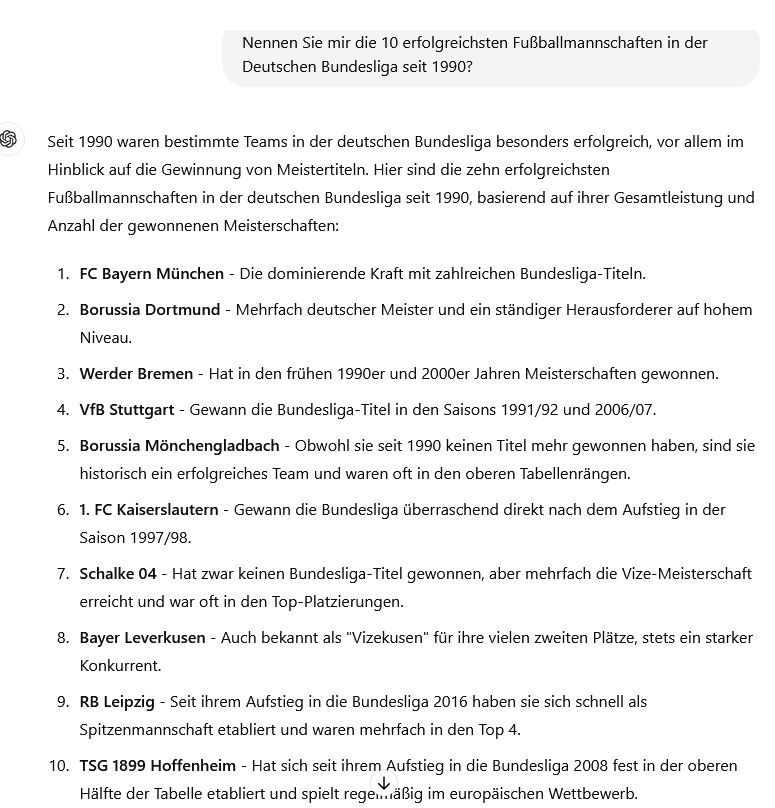
\includegraphics[width=0.7\linewidth]{Übung 3/Lösung/1_ 10 TOP Fussballtteams_seit_1990.png}
                    \caption{Top 10 Fussballmannschaften (genderneutral formuliert)}
                    \label{fig:top-teams}
                \end{figure}
    
                \begin{figure}
                    \centering
                    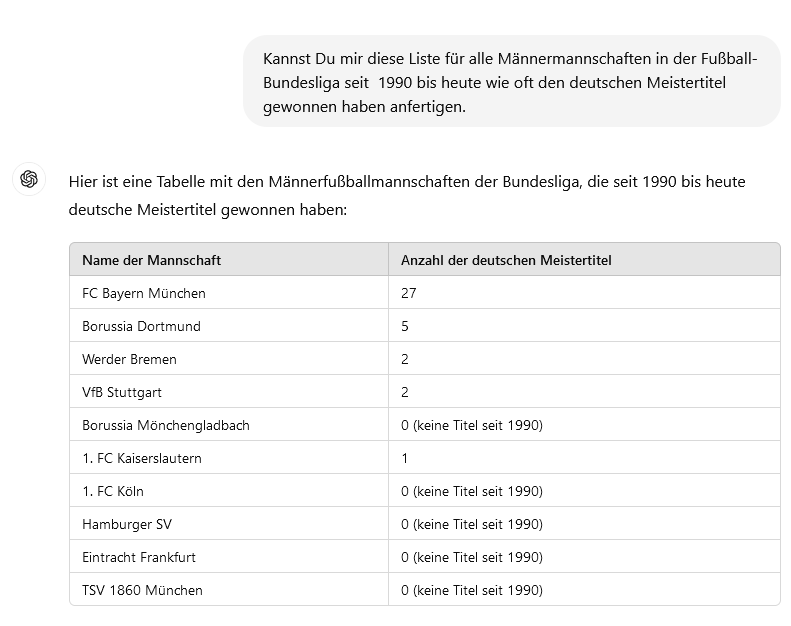
\includegraphics[width=0.7\linewidth]{Übung 3/Lösung/3_TOP_Teams Männer_seit_1990.png}
                    \caption{Erfolgreichste Männermannschaften}
                    \label{fig:top-maenner}
                \end{figure}
    
                \begin{figure}
                    \centering
                    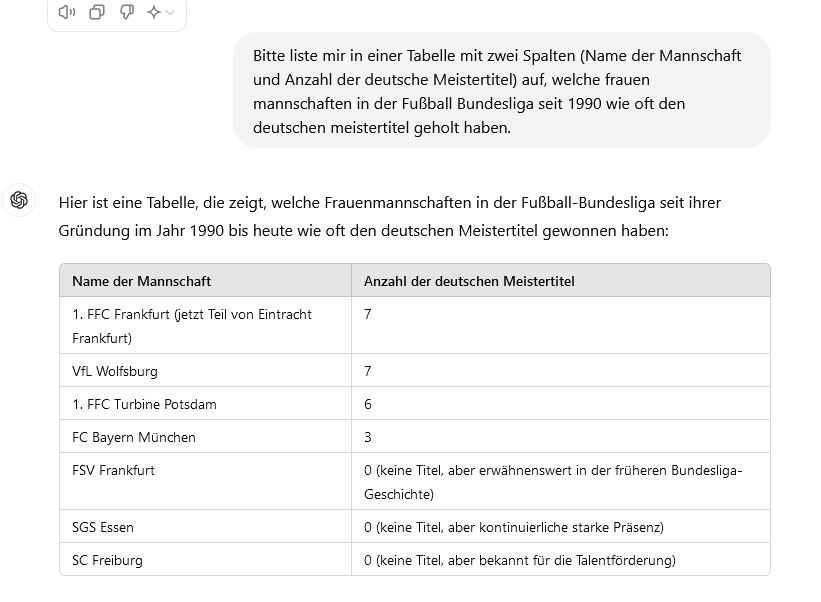
\includegraphics[width=0.7\linewidth]{Übung 3/Lösung/2_TOP Teams Frauen_seit_1990.png}
                    \caption{Erfolgreichste Frauenmannschaften}
                    \label{fig:top-frauen}
                \end{figure}
    
                \begin{itemize}
                    \item Ungleicheit historischer Daten: Historisch gesehen exisitieren fast 30 Jahre mehr Daten in der Männer Bundesliga (Männer-Bundesliga seit 1963, Frauen-Bundesliga erst seit 1990)
                    \item Gesellschaftlicher Bias: Bundesliga der Männer ist viel populärer, dadurch mehr Präsenz in der Gesellschaft
                    \item Ungleichheit aktueller Daten: Bundesliga der Frauen ist kleiner als bei Männern; selbst bei gleicher Berichterstattung pro Spieltag in einer Saison finden bei den Frauen weniger Spiele statt, über die berichtet werden könnte
                \end{itemize}
    
            \item Welche Folgen können Bias haben? Bringen Sie zwei Beispiele.
            \begin{itemize}
                \item 1. Justiz: Beeinflussung von lebensverändernden Entscheidungen für Betroffene
                \begin{itemize}
                    \item COMPAS-System, das in einigen US-Bundesstaaten eingesetzt wird, bewertet das Rückfallrisiko inhaftierter Personnen anhand von über 100 Variablen
                    \item Studie hat Bias herausgefunden, dass für die Risikobewertung die Hautfarbe einen großen Einfluss hat (irrtümlich werden Menschen mit schwarzer Hautfarbe doppelt so häufig mit einem hohen Risiko eingestuft; die Rückfallwahrscheinlichkeit von Menschen mit weißer Hautfarbe dagegen würde unterschätzt)
                    \item Quelle: https://www.amnesty.at/zukunftmenschenrechte/kuenstliche-intelligenz-und-menschenrechte
                \end{itemize}
                \item 2. Medizin: Falsche Diagnose
                \begin{itemize}
                    \item Beispiel Symptomchecker Apps: basieren oft auf klinischen Studien, für die meist junge Männer als Testpersonen genommen wurden (keine Gefahr der Schwangerschaft, weniger hormonelle Schwankungen)
                    \item dies führt dazu, dass bei der Diagnose Frauen oft übertherapiert werden (Überdosierung)
                    \item ZDFheute Nachrichten Interview mit Frau Prof. Dr. Sylvia Thun ab Minute 14 hier:
                    https://www.youtube.com/watch?v=NDD-jFioE4Q
                \end{itemize}
            \end{itemize}
            
            \item Erläutern Sie das Phänomen „Halluzination“ von LLMs. Erklären Sie wirksame Strategien, diesem zu begegnen.\
            \begin{itemize}
                \item LLMs erzeugen falsche Informationen; dies können Abweichungen von externen Fakten, kontextueller Logik oder beidem sein
                \item Strategie zur Miniminierung von Halluzinationen aus Nutzersicht:
                \begin{itemize}
                    \item Qualitativ hochwertiges Prompting: klare \& spezifische Anforderungen (Begrenzung der möglichen Ausgaben, relevante Datenquellen zur Verfügung stellen z.B. Promt beginnen mit „Gemäß Wikipedia….“, dem Modell eine Rolle vorgeben)
                    \item Es sollte darauf geachtet werden, dass der Eingabekontext konsistent und widerspruchsfrei ist
                    \item Few-Shot-Prompting
                    \item Bei Zweifel an den Ergebnissen bzw. zur Sicherstellung der Richtigkeit andere Informationsquellen zu Rate ziehen (Check your facts)
                \end{itemize}
                \item Anmerkung: Halluzinationen lassen sich allerdings niemals vollständig vermeiden
            \end{itemize}
        \end{enumerate}

    
    \section{Deep Fakes}
        Wie können Sie sich vor Deep Fakes schützen? Entwickeln Sie eine Strategie, wie Sie Deep Fakes besser erkennen können.
        \begin{itemize}
            \item Überprüfung des Kontextes: passt Aussage einer Person des öffentlichen Lebens zu ihrem/seiner sonstigen Positionierung? Folgt eine Stellungnahme der Person im Nachgang zu DeepFake?
            \item Kritische Begutachtung des Medieninhaltes: Wie wirkt dies auf Sie? Unscharfe Bereiche, Lippenbewegung, passen Mimik \& Gestik zum Kontext
            \item Quellenprüfung: wie vertrauenswürdig ist die Informationsquelle? Ist der gleiche Medieninhalt auch bei anderen Quellen zu finden?
            \item Selbststudium: Suchen Sie regelmäßig nach aktuellen DeepFakes, um sich selbst zu schulen, was mit aktueller Technologie möglich ist.
            \item Soziales Netzwerk: Tauschen Sie sich mit anderen Menschen in Ihrem Umfeld aus, holen Sie andere Meinungen ein und diskutieren einen potentiellen DeepFake.
        \end{itemize}

    
    \section{Rechtliche Aspekte}
        Was sind die wichtigsten Fakten zum EU AI Act (Stand der Gesetzgebung, Ziele des Gesetzes, Herangehensweise, Besonderheit)? 
        \begin{itemize}
            \item Stand der Gesetzgebung: Endphase des Gesetzgebungsverfahrens; Zustimmung des EU-Parlamentes am 13.03.2024, aktuell:  Überprüfung der Verordnung \& Übersetzung in alle Amtssprachen
            \item Ziele:
            \begin{itemize}
                \item Einerseits klare Anforderungen und Pflichten an KI-Entwickler \& -Deployer adressieren
                \item Andererseits sollen dadurch die Sicherheit, Grundrechte \& Gesundheit der Menschen geschützt werden
                \item Förderung von Innovation \& Wettbewerb
            \end{itemize}
            \item Herangehensweise ist ein risikobasierter Ansatz: Klassifizierung von KI in Risikoklassen (minimal, limited, high, unacceptable)
            \begin{itemize}
                \item Je nach Risikoklasse treten die Regelungen zeitlich gestaffelt in Kraft
                \item Beispiel: 6 Monate nach Inkrafttreten der Verordnung werden KI-Systeme der Risikoklasse unacceptable risk verboten
            \end{itemize}
            \item Besonderheit: Regelwerk gilt als historisch, da erstes KI-Gesetz weltweit
        \end{itemize}

    
\end{document}
